\chapter[Results]{Results}
Per research question a section is dedicated, describing the results. The final critical walkability factors are given in section \ref{Rrq1} The average walking speed of elderly, the outcome of the pedestrian area classification and the slope are presented in section \ref{Rrq2a}. In section \ref{Rrq2b} the surface signatures and comparison with surfaces from Matthews is presented. The last section \ref{Rrq2c} opens with a change-point method comparison, were after it presents per route a map with the derived change-points. 

\section{Results RQ 1. - Finding the critical factors for walkability}\label{Rrq1}
Critical walkability factors are found in literature and several interviews. The final list is presented in section \ref{Rfinallist}.

\subsection{Findings critical factors from literature}
Table \ref{tliteraturefinding} shows a summary of the occurrence of walkability criteria in literature \cite{ Bernhoft2008, Verschuur2013, Dunbar2004, Wennberg2010, Borst2008, Rosenberg2012, Vine2012, Matthews2003, Hovbrandt2007, WWT2012, Wennberg2009, Stahl2008, Stahl2013}, per category and level. The criteria are counted double if found multiple in different literature pieces. As can be seen in the table, most reports mentioned criteria that can be found on pavement level and criteria falling into the category of route attractiveness. \newline

\begin{table}[h]
\centering
\caption{Amount of critical walkability factors cound in literature. \label{tliteraturefinding}}
\begin{tabular}{|p{52pt}|p{45pt}|p{45pt}|p{45pt}|p{50pt}|p{45pt}||p{45pt}|}
\hline
\multicolumn{1}{|l|}{\multirow{2}{*}{Category}} & \multicolumn{5}{|m|}{Level} & \multicolumn{1}{|l|}{\multirow{2}{Total per \newline category}}\\ \cline{2-6}
& Crossing & Pavement & Street & Environment & Weather & \\
\hline
Accessibility 	& 9 & 20 & 3 & 8 & 0 & 40 \\
Quality 		& 4 & 24 & 4 & 0 & 0 & 21 \\
Obstruction		& 1 & 20 & 0 & 0 & 0 & 21 \\
Route Attractiveness & 1 & 7 & 17 & 21 & 11 & 57 \\
Safety			& 8 & 0 & 10 & 4 & 0 & 22 \\
\hline \hline
Total per level & 23 & 71 & 34 & 33 & 11 & 172 \\
\hline
\end{tabular}
\end{table}

In the next table, a more detailed overview of the walkability criteria found on pavement level is given with detailed characteristics of pavement and objects, which were found most. The two detailed walkability criteria mentioned most are: irregular surfaces and (wrongly) parked bikes and cars. 

\begin{table}[h]
\centering
\caption{Detailed overview of criteria at pavement level. \label{literaturepavement}}
\begin{tabular}{|p{135pt}|p{45pt}||p{135pt}|p{45pt}|}
\cline{1-2}
Sub-Categories & Count \\
\cline{1-2} \cline{1-2} \cline{3-4}
\multirow{6}{135pt}{Criteria about the pavement (availability and quality)} & \multirow{6}{*}{ 22 } & Detailed criteria & Count \\ \cline{3-4}
& & Presence of pavement & 4 \\
& & Too wide or narrow pavement & 3\\
& & Irregular surface & 13 \\
& & Slope & 2 \\
\cline{3-4}
& & Total & 22 \\
\hline

Criteria about curbs and ramps & 12 \\
\cline{1-2}
Stairs precense and quality & 10 \\
\hline
\multirow{6}{*}{Objects in the way} & \multirow{6}{*}{ 20 } & Detailed criteria & Count \\ \cline{3-4}
& & Parked bikes, cars, scooters (temporary) & 8 \\
& & Physical stationary objects (poles trees ect.) & 5\\
& & Pavement objects (gutters) & 3 \\
& & Temporary objects (commercial signs, branches) & 4 \\
\cline{3-4}
& & Total & 20\\
\hline
Unatractive objects (litter, poop, garbage, graffiti) & 7 \\
\cline{1-2} \cline{1-2}
Total & 71 \\
\cline{1-2} 
\end{tabular}
\end{table}



% %Pavement suitability

% This will include the availability of a pavement, the minimum width, the surface material, the presence of curbs and ramps, slope.
% Standard pavement should be $1.2m$, excluding the curb. In intensively used pavement, around schools, shops etc., the width should be around $1.8m$. Narrow pavements are $0.9m$, excluding curb. Verschuur

% Verschuur already did a study on these factors defining

% is information a classification can be made on the pavements on how suitable they are, like Verschuur:
% All pavements with a with smaller than 1.2 m are assigned as not suitable. All pavements in intensively used areas, smaller then 1.8m are also assigned not suitable. 
% All pavements wider or equal to 1.2 in standard areas are positive
% All pavements wider or equal to 1.8 in intensively used areas are positive.
% All pavements wider or equal to 1.8 in standard areas are very positive.
% As an example, Figure 6 shows a map from Verschuur on pavement width analysis in combination with presence of barriers. 

% Figure 6 Example pavement suitability from (Verschuur, 2013


% Positive objects
% Route attractiveness
% land use mix
% Overall street suitability and environmental influences
% Street connectivity
% Traffic density
% Pavement density

\subsection{Summary personal interviews}
\textbf{Participant 1} uses a wheeled walker already for 8 years. Without it she loses balance and so is really depended on the rollator. Short distances however are done often without the rollator but would be safer with. Although she has severe fright of falling, she walks outside at least once a day for half an hour to stay fit. But she would rather stay at home. Because when she gets tired her ankles weaken and she is even more afraid of falling. For her, if the pavements would be more smooth, she would be able to walk much further because it is more easy and she would not get tired that quickly. Loose tiles, pits, wrongly parked cars, tourists, sloping pavements are a problem to her. Also the amount of people on the street is something she tries to avoid. In conclusion, walking is not a relaxing activity for her.

\textbf{Participant 2} is a real outdoor walker. She goes out on the streets several times a day and strolls around the whole neighbourhood. She uses the rollator for several years and feels that the rollator is really easy and a blessing for her. It keeps her mobile and enjoy Amsterdam around her. The problems mentioned by her are the uneven tiles or half loose tiles. So not well maintained pavements. Also when cars are parked wrongly it makes her move off the high curbs which is difficult. After asking for resting benches she mentioned that the hight of the resting benches are too low. So if she would sit on these she would have difficulty getting up again. She was really positive about the people on the street, in her perception they are friendly and helpful. Also she attached a bell on her rollator, so that if someone is in the way she would just ring the bell and she can pass. 

\textbf{Conclusion.} Most often named: 
\begin{itemize}
\item Irregular surfaces as in loose tiles or bad maintenance. 
\item Sloping surfaces
\item Wrongly parked cars
\end{itemize}


\subsection{Summary interviews at Rollator Loop}
The age of the participants at the Rollator Loop ranged from 77 to 94. Some used the rollator for more than 6 years, while others only since half a year. When starting using a rollator, participants said they did not dare to walk without it any more, because of fear of falling. Most of them mentioned grocery shopping as the main activity for using a rollator outdoors, for it is easy to put the groceries in. 
Participants and their accompaniments said that you only notice the bad quality of the streets when your mobility worsens and you start needing a rollator to help you. Problems mentioned were; roots of trees make the pavement uneven, pavements are convex and these sloping circumstances need you to adjust the rollator all the time. The maintenance is not sufficient. Not nicely finished pavements, transition from tiles to asphalt not even, public transport stops not adjusted or tram rails. Sloping pavements and bad maintenance as in uneven surface, were mentioned several times. Positively mentioned was that there is enough space to walk. Not all participants have difficulty with going on and off the pavement. One participant did not have any problems while walking on the street while walking to the grocery store across the street a few times per week. 

\textbf{Conclusion.} Most often named: 
\begin{itemize}
\item Irregular surfaces as uneven pavements or bad maintenance. 
\item Uneven transition of road segments.
\end{itemize}


\subsection{Findings policy perspective}

From the interviews with members of the Amsterdam municipality, working on Transport and Public Space, we learned that the pedestrian is not a main focus for the design in the public space. In Amsterdam the focus goes to the growing number of tourist in the centre and on accessibility of public transport and public buildings. Interventions done to increase accessibility for pedestrians to public transport, all public transport stops are raised for easier entrance into the bus and trams. In order to avoid cars parking on the pavement, post are placed on the edge and curbs raised. For the future, the municipality is working on a new framework for pedestrians, as part of the project, Sailing and Transport in the Puclic Space. The first stage to be completed at the end of 2015. The framework will include the design policy for public space with principals, assumptions, guidelines, goals, test and products. All to make the pedestrian more visible, measurable and comparable. It will be a integrated pedestrian policy, covering everything to do with pedestrians, from crowd management to accessibility.
The goal is to grow and give more space for pedestrians and increase the use of the public space. This new design is part of the restructuring inside the municipality. Before the policy design for the public space was scattered over districts, now it is brought back to one central governmental body inside the municipality.

When informing to existing geodata about pedestrian area, surface material and curb locations, nobody could tell exactly what and where the data was and if, even existed. There is use of geodata at the municipality, though nobody could tell exactly what. 

% More post placed and raised pavements, to avoid cars on the pavement.
% Public transport stops are raised for easier entrance into the bus and trams. 
% Puccini method as design policy for public space. 
% GIS data available but not sure what. 
% Centre, tourist are the main problem. 
% More ageing. Accessibility is getting a problem. Living independent is policy. There is still a lack at the municipality in providing facilities and care. 
% Mostly focus on accessibility of public transport and public buildings. 
% More people walk. 
% Putting up a new framework for pedestrians. First stage to be completed end of 2015. The framework includes the design policy for public space with design principals, assumptions, guidelines, goals, tests, and products. 
% Integrated pedestrian policy, covering all from crowd management to accessibility. 
% Indicators should be, measurable so quantitative but also qualitative.

The policy documents collected are:
\begin{itemize}
\item Leidraad centrale verkeers commissie Amsterdam (2011) Team Infrastructuur Stad, Municipality of Amsterdam ~\cite{leidraad2011}
\item Structuurvisie Amsterdam 2040 Economisch sterk en duurzaam (2011) Municipality of Amsterdam ~\cite{Bossink2011}
\item Amsterdam aantrekkelijk en bereikbaar, Mobiliteits Aanpak Amsterdam 2030 (2013) Municipality of Amsterdam ~\cite{Kuik2013}
\item Amsterdam in cijfers 2014 (2014) Department research and statistics, Municipality of Amsterdam ~\cite{Hylkema2014}
\item Senioren en Langer zelfstandig wonen. (2014) Department Wonen Zorg en Samenleven, Municipality of Amsterdam ~\cite{Booi2014}
\end{itemize}

Provided by the municipality is:
\begin{itemize}
\item Handboek Puccini methode Inrichting openbare ruimte onderdeel verharding (2014) Municipality of Amsterdam ~\cite{puccini2014}
\end{itemize}

A document Leidraad of 2011~\cite{leidraad2011} contains guidelines for the Central Traffic Commission in Amsterdam and provides a lot of guidelines in the public space for the pedestrian. The following guidelines are given especially for the pedestrian area:

\begin{itemize}
\item A minimum free passage width of 1.50$m$ is necessary. 
\item If pedestrian use is very high, the minimum free passage width of 2.50$m$ is necessary.
\end{itemize}

In practice a lot of extra space is needed to place all street furniture. Therefore an extra space of 0.5$m$ has to be added as 'smart' strip to place lanterns, poles, benches, garbage containers etc. Preferably 1$m$ if shops have protruding displays at the building side. An extra 1.80$m$ is needed when bike racks are placed on the pavement.~\cite{leidraad2011} For more research on this topic, Verschuur 2013, looked at these guidelines in a case study in Utrecht.~\cite{Verschuur2013}

The following guidelines are given in the Leidraad~\cite{leidraad2011} especially for mobile impaired pedestrian:
\begin{itemize}
\item For mobile impaired, especially with a wheelchair with accompanist a desired obstacle free walking space is required of 2 meter.
\item The slope to be applied cannot be steeper then 1:25 (4\%)
\item Big heiht difference have to be solved with elevators 
\end{itemize}

Several policy guidelines for pedestrians are found in the documents for Amsterdam:

\begin{itemize}
\item More safety for the pedestrian~\cite{Bossink2011}
\item More space for the pedestrian~\cite{Bossink2011}
\item in the centre of Amsterdam, give the pedestrian the most safe and attractive public space with the least amount of obstacles and delay.~\cite{Kuik2013}
\item Inside the highway ring, provide wide pavements and safe crossings.~\cite{Kuik2013}
\item Design more logical, straight, obstacle free ongoing walking routes on the pavement~\cite{puccini2014}
\item Reduce hight differences in tile work and minimize the use of stairs and ramps in the public space.~\cite{puccini2014}
\end{itemize}

\subsection{Final list critical factors}\label{Rfinallist}
The top 3 critical factors that decrease walkability derived from all of the above are: 
\begin{enumerate}
\item Wrongly parked bikes and cars
\item Sloping pavement
\item Irregular pavement
\end{enumerate}

The first item will not be examined, for parked bikes and cars are temporary obstacles which can be hard to detect through stationary geo data. The applicability of Geo information systems for monitoring wrongly parked bikes and cars is a whole new study on its own.

\section{Results RQ 2 - Collection and analysis of available geodata}\label{Rrq2a}
\subsection{Average walking speed}\label{Rrq1b}
Based on the Rollatorloop of 2014 and 2015, an average walking speed of 4.62$km/h$ was found. The routes walked all started in the athletics track in the Olympic stadium.
The 400$m$ was only using the athletics track so had an extreme good, flat and regular surface.
The 1000$m$ route went round outside the stadium over the street and pavement, so had a less smooth surface. The third route 2500$m$ even went through a park with soft gravel, so had the least best surface but was acceptable for rollator users. 
Overall the weather conditions were extreme good. 
In the table \ref{statistiswalkingspeed} and figure \ref{averagewalkingspeed} can be seen that the average walking speed decreases when walking longer distances. 
The total number contains all participants labelled as male, female or unknown. Therefore, the sum of male and female differences from the total number.

\begin{figure}[h]
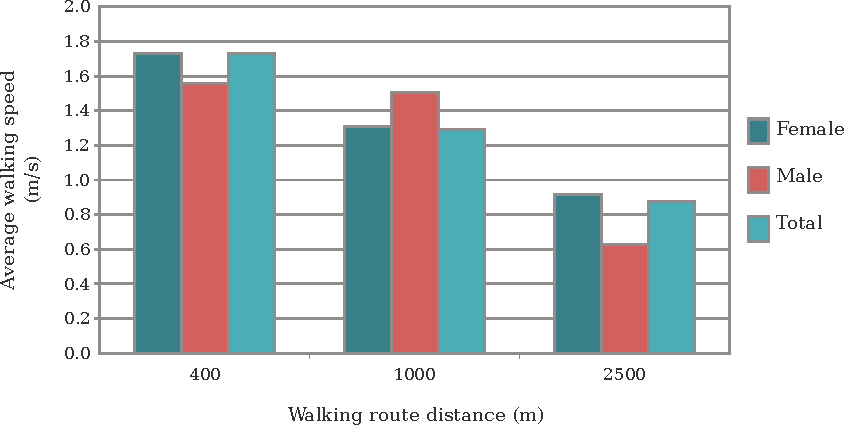
\includegraphics[width=\textwidth]{img/R_averageWalkingSpeed.pdf}
\centering
\caption{Average walking speed of the participants from the Rollatorloop (2014 and 2015). \label{averagewalkingspeed}}
\end{figure}

\begin{table}[h]
\caption{Average walking speed of the participants from the Rollatorloop (2014 and 2015) \label{statistiswalkingspeed}}
\centering
\begin{tabular}{|p{70pt}|p{70pt}|p{70pt}|p{70pt}|p{70pt}|}
\hline
Distance & Sex & Count & $m/s$ & $km/h$ \\
\hline
400 & Male	 & 25	& 1.56 & 5.60 \\
400 & Female & 97	& 1.73 & 6.23 \\
% 400 & Total	 & 134 & 1.73 & 6.23 \\
\hline
1000 & Male		& 5	 & 1.51	 & 5.42\\
1000 & Female	& 28 & 	1.31 & 4.72\\
% 1000 & Total	& 37 & 	1.29 & 4.65\\
\hline
2500 & Male		& 1	 & 0.63	 & 2.26\\
2500 & Female	& 7	 & 0.91	 & 3.29\\
% 2500 & Total	& 8	 & 0.88	 & 3.16\\
\hline
& Total & 179 & 1.30 & 4.62 \\
\hline
\end{tabular}
\end{table}


\subsection{Determining pedestrian area with the GBKA}
The GBKA was used to determine how much surface is determined for pedestrians, the road segments are given a new attribute with our own classification: 1 for transport, 2 for pedestrian area and 3 unpaved areas. In annex \ref{Ajordaan} the total area of the Jordaan is shown with our derived classification. Here, a detailed map shows of an area where the classification turned out to be almost correct, but also contains streets segments that are wrongly assigned as pedestrian area. In total, the Jordaan has around 300000$m^2$ of public road surfaces. About 53\% of this is intended for pedestrians according to the developed approach. This share of road does contain poles, lanterns, bicycle racks, parking lots and all other street furniture. 

Figure \ref{jordaanroad} shows in blue the pedestrian area as conducted. The street Tweede Boomdwarsstraat is wrongly classified as well as most bridges. The parking lots in the centre of the road Westerstraat are labelled as pedestrian area but are not suitable for pedestrians as it is full with cars and other street furniture. See Figure \ref{westerstraat} image from Google street view of the Westerstraat. 
\renewcommand{\arraystretch}{1.5}
\renewcommand{\tabcolsep}{0.2cm}
\begin{table}[h]
\caption{Road segment classification outcome. \label{statroadsections}}
\centering
\begin{tabular}{|p{125pt}|p{125pt}|p{125pt}|}
\hline
Road Section & Total Area	& Percentage\\
\hline
All Road Sections & 293317.25 & 100.00\\
\hline
1. Transport & 133789.66 & 45.61\\
2. Pedestrians & 156159.49 & 53.24\\
3. Unpaved	& 3368.1 & 1.15\\
\hline
Below 4\% slope & 114341.08 & 38.98\\
Pedestrian below 4\% slope & 24466.67 & 8.34\\
\hline
\end{tabular}
\end{table}


\subsection{Mapping sloping surfaces with AHN data}
In table \ref{statroadsections} from the previous section, also the area of pedestrian area with a slope lower then 4\% and the total area below 4\% slope is given. Those are consecutively, 8\% and 39\% of the total area.
The top part of figure \ref{jordaanroadslope} the Westerstraat can be seen with the slope below 4\% in green. The roads destined for cars mostly show green colour except for the speed bumps which can be clearly distinguished. The pedestrian area on the other hand contains more red spots. The bottom part of figure \ref{jordaanroadslope} shows the average slope per road section polygon. Mostly the car area (1) stays below the 4\% mark while the pedestrian area (2) has higher slopes. Curbs and objects placed on the pavement give a hight slope value and fall in the pedestrian polygons. Building edges which are not cleaned away well enough can give a wrong impression of the pedestrian polygons. The original hight map of the AHN2 can be found in Annex \ref{AAHN}.

% The AHN2 promised good possibilities to detect surface quality and sloping pavements. Even the detection of curbs and ramps could be possible.

\begin{figure}[ht]
\includegraphics[width=\textwidth]{img/R_jordaan.pdf}
\centering
\caption{Detail segment classification in the Jordaan(Westerstraat).\label{jordaanroad}}
\end{figure} 

\begin{figure}[hb]
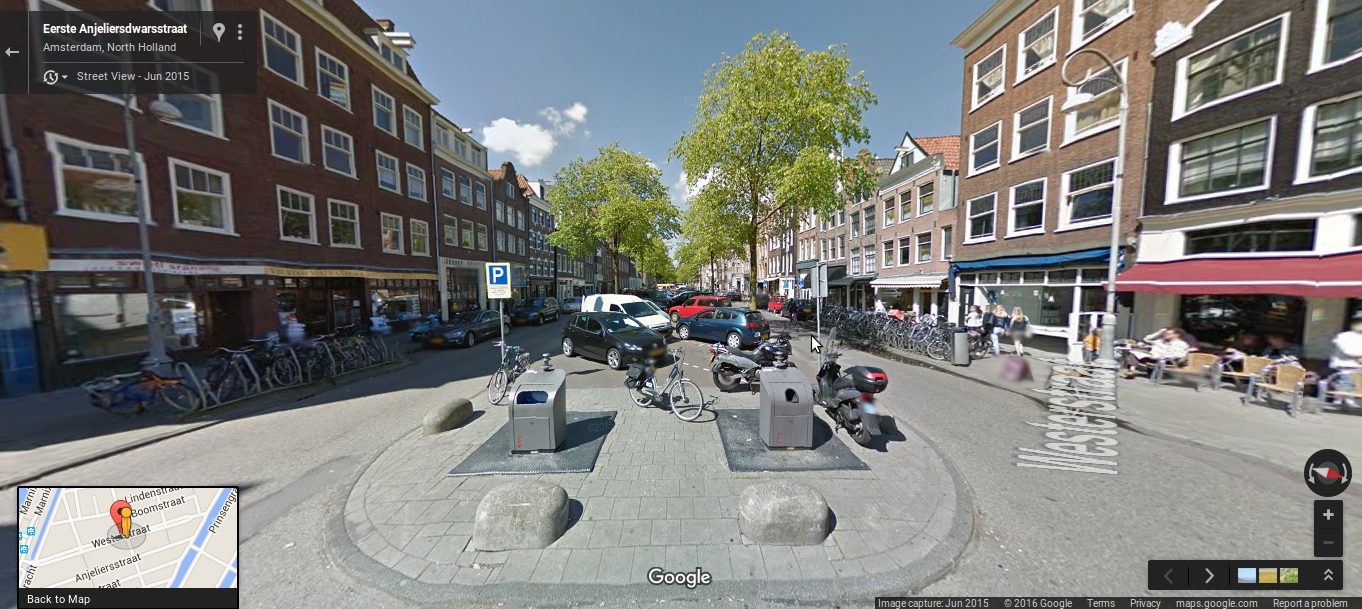
\includegraphics[width=\textwidth]{img/R_Westerstraat.png}
\centering
\caption{Google Street View image of the Westerstraat.\label{westerstraat}}
\end{figure} 

\clearpage
\begin{figure}[h]
\includegraphics[width=\textwidth]{img/R_slope.pdf}
\centering
\caption{Detail of slope and average slope per road section in the Jordaan(Westerstraat).\label{jordaanroadslope}}
\end{figure} 
\clearpage
\section{Results RQ 3- Collection of geodata of rollator movements and analysis}\label{Rrq2b}
\subsection{Mapping irregular surfaces with an Accelerometer}
Figure \ref{figsurfaces} shows the accelerometer output of the $z-axis$ per measured surface. The exact statistical summary of every surface is given in table \ref{surfacehindrance} containing the $z-axis$ acceleration mean, standard deviation, the variance, the minimum and maximum, first and third quantile and the median. The median and mean are roughly the same for every surface, because the accelerometer measures acceleration in the vertical direction around 1$m/s/s$, which is equal to gravity. Any acceleration aiming up will also go down. The extent of acceleration a surface causes in the vertical direction, the standard deviation or variance, tells more about the differences in surface.
The box plots \ref{boxhindrance} show the differences in variance per surface. A clear difference per surface type can be seen. The smooth concrete, gave almost no acceleration in the vertical direction, while stones or grass showed more vibration and so higher and lower values in minimum and maximum as well as the standard deviation and variance. 

% mss nog plaatje van de GPS tracks locaties en de gekoppelde data? 
\begin{figure}[H]
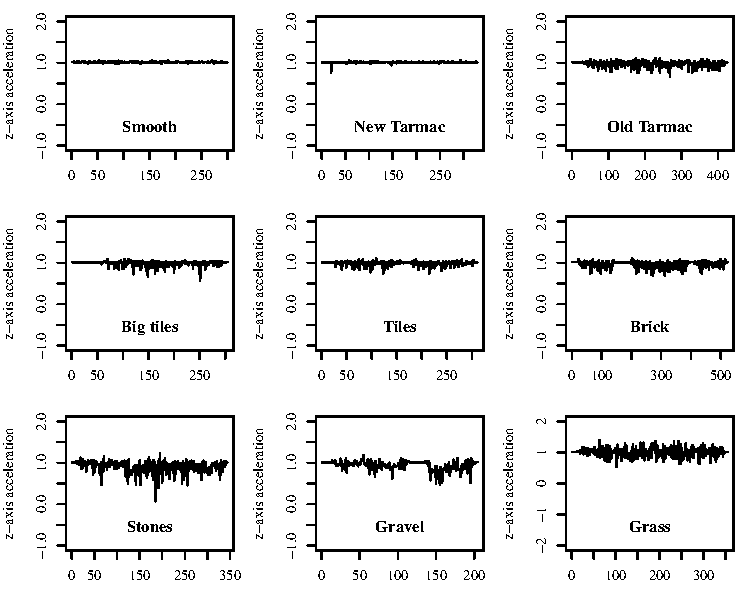
\includegraphics[width=\textwidth]{img/R_AllsurfaceGraphs.pdf}
\centering
\caption{Accelerometer output of the z-axis per surface type.\label{figsurfaces}}
\end{figure} 

\begin{table}[ht]
\caption{Statistical summary of z-axis acceleration per surface type. \label{surfacehindrance}}
\centering
\begin{tabular}{|p{46pt}|p{30pt}|p{30pt}|p{30pt}|p{30pt}|p{30pt}|p{30pt}|p{30pt}|p{30pt}|}
\hline
Surface: & Mean & Std dev & Variance & Min & Q1 & Median & Max & Q3\\
\hline
Smooth & 1.02 & 0.02 & 0.00 & 0.97 & 1.02 & 1.06 & 1.01 & 1.03 \\
New tarmac & 1.01 & 0.02 & 0.00 & 0.77 & 1.01 & 1.06 & 1.01 & 1.02\\
Old tarmac & 0.97 & 0.07 & 0.01 & 0.67 & 0.99 & 1.12 & 0.94 & 1.02\\
Big tiles & 0.99 & 0.07 & 0.00 & 0.58 & 1.01 & 1.10 & 0.98 & 1.02\\
Tiles & 0.99 & 0.06 & 0.00 & 0.74 & 1.01 & 1.10 & 0.97 & 1.02\\
Brick & 0.96 & 0.07 & 0.01 & 0.68 & 0.98 & 1.11 & 0.92 & 1.01\\
Stones & 0.91 & 0.14 & 0.02 & 0.07 & 0.94 & 1.23 & 0.84 & 1.01\\
Gravel & 0.94 & 0.12 & 0.02 & 0.48 & 0.97 & 1.19 & 0.87 & 1.01\\
Grass & 1.01 & 0.15 & 0.02 & 0.54 & 1.02 & 1.40 & 0.93 & 1.10\\
\hline
\end{tabular}
\end{table}

\begin{figure}[hb]
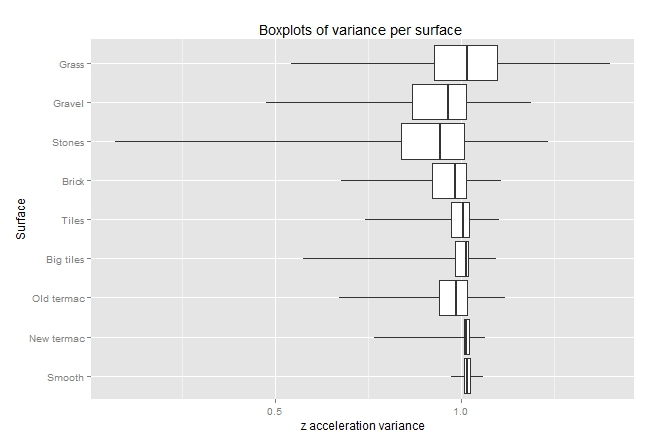
\includegraphics[width=\textwidth]{img/R_Surfaces_Variance.jpeg}
\centering
\caption{Box plots showing the variance per surface type.\label{boxhindrance}}
\end{figure} 

% \begin{figure}[ht]
% 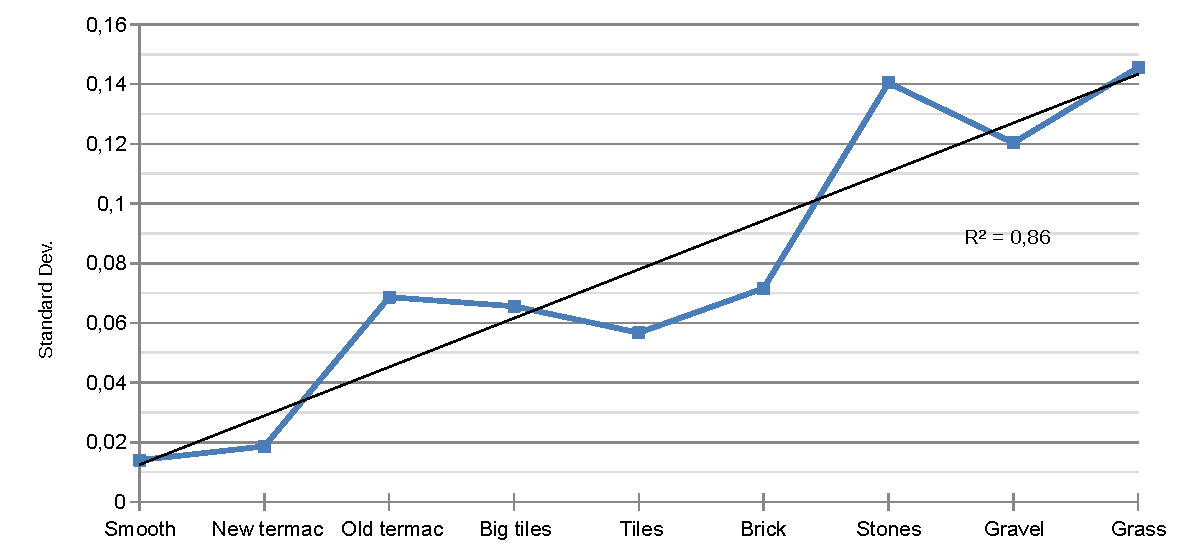
\includegraphics[width=\textwidth]{img/R_statistics_surfaces2.pdf}
% \centering
% \caption{The surface hindrance standard deviations with the regression line \label{hindrance2}}
% \end{figure} 
% \clearpage
\clearpage

\subsection{Comparison with Matthews et al. 2003}
The standard deviation values of the surfaces are converted to relative scores. The value 1 is assigned to the smooth surfaces as basis. The other values are calculated as a factor from this. Lower scores represent levels of least hindrance while higher scores represent high levels of vibration and more hindrance. These factors are compared with the results of a similar study by Matthews et al.(2003) and matched upon the surface description. The factors from Matthews et al. do differ in value but are also calculated relatively to its most smooth surface, concrete. When plotting both values against each other a correlation coefficient of 0.75 is found. This indicates a positive but moderate correlation between the two data sets. This proves that the surface coarseness or irregularity can be determined with an accelerometer. 

\begin{table}[hb]
\caption{Relative scores of surface hindrance as measured and from Matthews et al. \label{compare}}
\centering
\begin{tabular}{|p{67.6pt}|p{55.6pt}|p{55.6pt}|p{55.6pt}|p{55.6pt}|p{55.6pt}|}
\hline
Surface & Standard Deviation of z-ax & Percentage & Factor & Factor given by Matthews & Surface name by Matthews \\
\hline
Smooth & 0.01 & 100.00 & 1.0 & 1 & Concrete \\
New tarmac & 0.02 & 132.72 & 1.3 & 1.3 & Tarmac\\
Old tarmac & 0.07 & 489.01 & 4.9 & &  \\
Big tiles & 0.07 & 467.30 & 4.7 & & \\
Tiles & 0.06 & 404.02 & 4.0 & 1.2 & Paving \\
Brick & 0.07 & 510.27 & 5.1 & 1.6 & Brick \\
Stones & 0.14 & 1000.62 & 10.0 & & \\
Gravel & 0.12 & 857.41 & 8.6 & 8 & Gravel \\
Grass & 0.15 & 1037.63 & 10.4 & 6 & Grass \\
\hline 
\end{tabular}
\end{table}

\begin{figure}[hb]
\includegraphics[width=\textwidth]{img/R_comparisonMatthews.pdf}
\centering
\caption{Comparison factors measured and factors given by Matthews et al.\label{comparefig}}
\end{figure} 

\clearpage



\section{Results RQ 4 - Mapping abnormal or change events with Accelerometer, GPS and AHN2 data}\label{Rrq2c}

\subsection{Comparing different changepoint detection methods}

First, the different changepoint detection methods and penalty values had to be tested to see which model approaches the most plausible result and approaches the truth the best. This was shortly done for all datasets. Here we will show possibilities of the acceleration output of the $z-ax$ of the rollator route in detail. See figure \ref{cpcomp} Walking with a speed of around 4$km/h$, the distance between each measured point is around 25$cm$ with a sample frequency of 5 points per second (Normal settings). The total route was 500 meter. 

The first method, finding changepoints for the variance with PELT method, resulted in 10 changepoints. So on average one changepoint per 50 meter. Some outlying peeks are missed by the model, and are not enclosed by changepoints, while they could indicate an unevenness in the surface. 

The second method variance with PELT $1.5*log(n)$ resulted in 69 points. On average one point per 7 meter. Now, the outlying peaks are enclosed by two changepoints, indicating exactly where a abnormality happens. Changing the penalty value solves the problem of under-fitting the model. 

Method BinSeg and BinSeg $1.5*log(n)$ took a longer computing time and resulted in only 5 changepoints for the variance. Method PELT and PELT $1.5*log(n)$ for the mean resulted in no changepoints. Method SEGNeigh on the mean of the variance didn't gave any output. The PELT method for both the mean and variance at the same time had 50 changepoints. 


Thus, for detecting changepoints in the variance of the acceleration the PELT method with a manual pen value of $1.5 * log(n)$ is used to overcome over and under fitting. For it showed the most plausible result.

A same kind of figure for the analysis of the best methods to detect changepoints in the speed dataset, can be found in annex \ref{Acptest}.
For the speed we look at changes in the mean.

Significant changes are, that the speed drops 2 times almost to the zero, the first drop is seen when walking up and down the pavement curb. The second drop coincides with a curve in the road where probably a short stop was made. The first method, finding changepoints for the mean with PELT method, resulted in 3 changepoints and missed the second drop in speed. The second method variance with PELT $1.5*log(n)$ resulted in more points and did detect the second drop in speed. Plus, it broke up the first stop into 3 parts. Method BinSeg, BinSeg $1.5*log(n)$ and SEGNeigh resulted in no output.The PELT method for both the mean and variance at the same time had made a break point on every value of a change in speed, therefore over-fitted the model. 
When looking at the changepoints in the variance, PELT and PELT $1.5*log(n)$, detected more changepoints. Sometimes giving a logical breakpoint, for example at the huge drop in speed. But it also detected multiple points really close to each other, singling out steps in gradual decrease or increase of speed over a longer distance. This gives too many points: every 5 meter. 


For every individual dataset, the best possible penalty settings are considered, for there can be a big difference in characteristics of the dataset for speed, slope and acceleration. Though, for all datasets, the PELT method was used, because of quick computing time and good accuracy and distribution of changepoints over the dataset. In general the slope datasets resulted in too much over-fitting, therefore a different penalty type was chosen, the AIC or the BIC model. For every dataset the model of fit is indicated in the summary tables of the next section. 





% ### Because of overfitting the model of speed a penatlyt type of BIC AIC or Hanan-Quinn can be chosen to solve the problem of overfitting.
% ## a penalty term for the number of parameters in the model; the penalty term is larger in BIC than in AIC.
% ##he penalty discourages overfitting (increasing the number of parameters in the model almost always improves the goodness of the fit).
% ## we use an adjusted penalty to overcome the problem of overfitting. The GPS contains abonormal peaks due to measurement errors. If a model is generated that fits too well, these are taken as truth. Using a penalty these extreme measurments are not taken into the analysis. These are plausibly artifacts of the data rather
% ## than true changes in the underlying process. In an effort to remove these seemingly spurious changepoints we can increase the penalty to 1.5 * log(n)
% ## The result seem more plausible. 

\begin{figure}[ht]
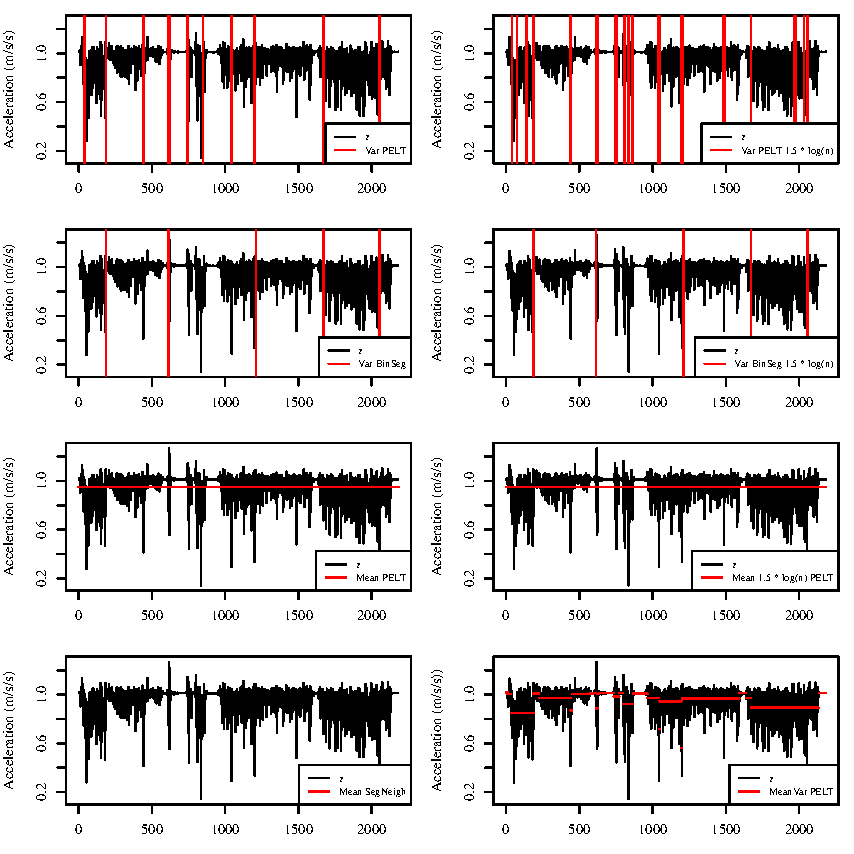
\includegraphics[width=\textwidth]{img/R_comparisonMethodsZ.pdf}
\centering
\caption{Comparison of different algorithms for changepoint detection in accelerometer z-axis output.\label{cpcomp}}
\end{figure} 

The next sections show the changepoints detected for average height, average speed, average slope, and variance of the total acceleration for all the measured routes. The changepoints are assigned to a location through linking its time stamp with the time of the GPS data. 

\clearpage

\subsection{changepoint and Segments found for the Meetrollator walking route}
In figure \ref{routeM} the route of the measurement rollator is shown with the detected changepoints indicated. The numbers show the time index that is the same as found in the graph \ref{routeR}, which shows the datasets with the changepoints and segments. The average walking speed was 1.2$m/s$ ($4.3km/h$).

\begin{figure}[ht]
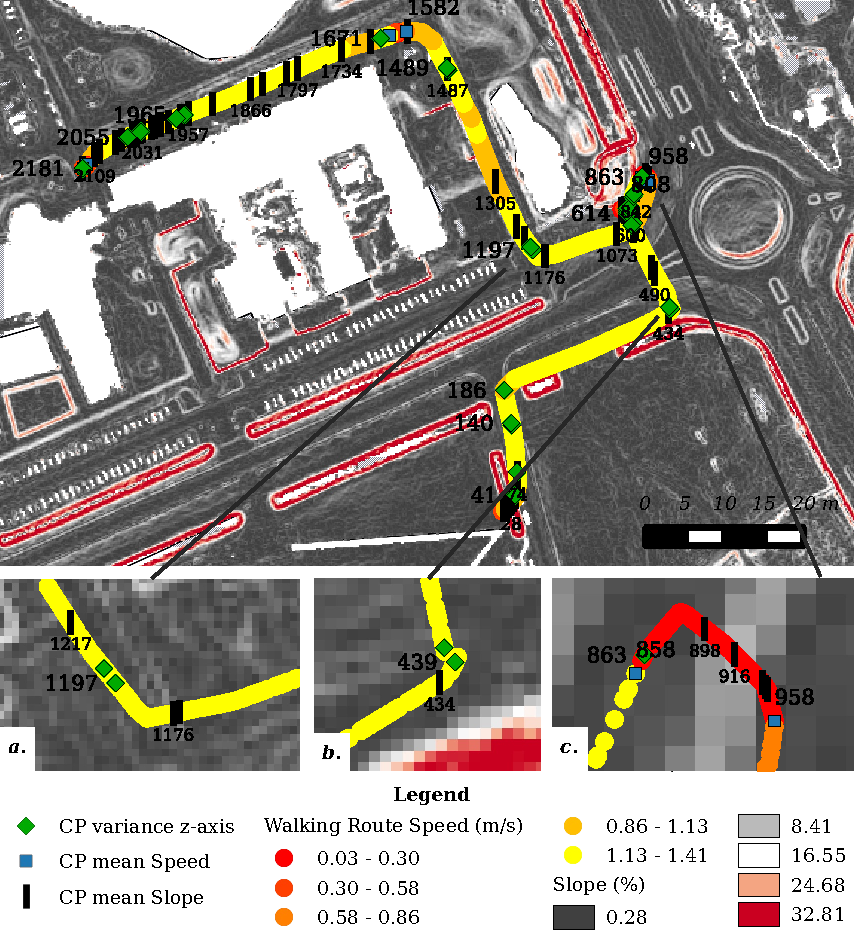
\includegraphics[width=\textwidth]{img/R_meetrollatorroute.pdf}
\centering
\caption{Map with changepoints of the Meet Rollator route.\label{routeM}}
\end{figure} 

\clearpage

The right zoomed in square (c) shows the area where a little detour was taken, walking down and up the curb again. The slope map clearly shows the location of the curb. The blue squares indicate a decrease and increase in speed while going over the curb. The black stripes are the slope changepoints, and could indicate the curb. One point in change of the vertical acceleration is detected. The left zoomed in square (a) shows again that the changepoint in slope is detected, where the black stripes and the slope map show a bump. Though the changepoint in the accelerometer fall slightly later in the route. The slope is derived from the location of the track, while the accelerometer is linked to the time stamp of the GPS. Because of GPS inaccuracy's these points do not have to fall at the same point in the route. The middle map (b) shows a peak in the vertical acceleration at time index 439. No speed changes are detected. Figure \ref{straatbocht} shows an image of the location. A obstacle in the pavement can be the cause of this peak in the vertical acceleration. Because the GPS is not accurately enough this is only an assumption. 

\begin{figure}[hb]
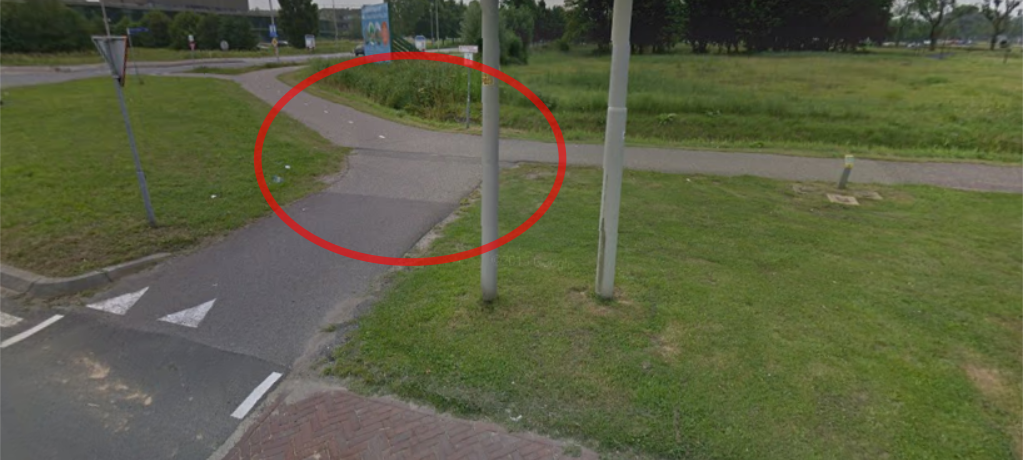
\includegraphics[ width=\textwidth]{img/R_bochtwageningenmeetrollator3.png}
\centering
\caption{The surface with obstacle from detail (b) figure \ref{routeM} \label{straatbocht}}
\end{figure} 

\renewcommand{\arraystretch}{1}

\begin{table}[hb]
\centering
\caption{Summary of changepoint output and methods used, per dataset, for the MeetRollator walking route.}
\label{summarymeetrollator}
\begin{tabular}{|p{70pt}|p{70pt}|p{70pt}|p{70pt}|p{70pt}|}
\hline
& Slope & Speed & Variance z-axis & Variance total \newline acceleration\\
\hline 
Changepoint type 	& Change in mean 	& Change in mean 	& Change in variance 		& Change in variance \\
Method of analysis	& PELT 				& PELT 				& PELT 						& PELT \\
Test Statistic 		& Normal 			& Normal 			& Normal 					& Normal \\
Type of penalty		& Manual with value \newline 11.53131 & Manual with value\newline 11.53131 & Manual with value\newline 11.53131 & MBIC with value\newline 23.06262 \\
Minimum Segment Length	& 1 			& 1 				& 2 						& 2 \\
Maximum no. \newline of cpts 	& Inf 			& Inf 			& Inf 						& Inf \\
Number of \newline changepoints 	& 69			& 7 				& 28 						& 12 \\
\hline
\multicolumn{5}{|l|}{Created Using changepoint version 2.2 } \\
\hline
\end{tabular}
\end{table}

\clearpage

\begin{figure}[ht]
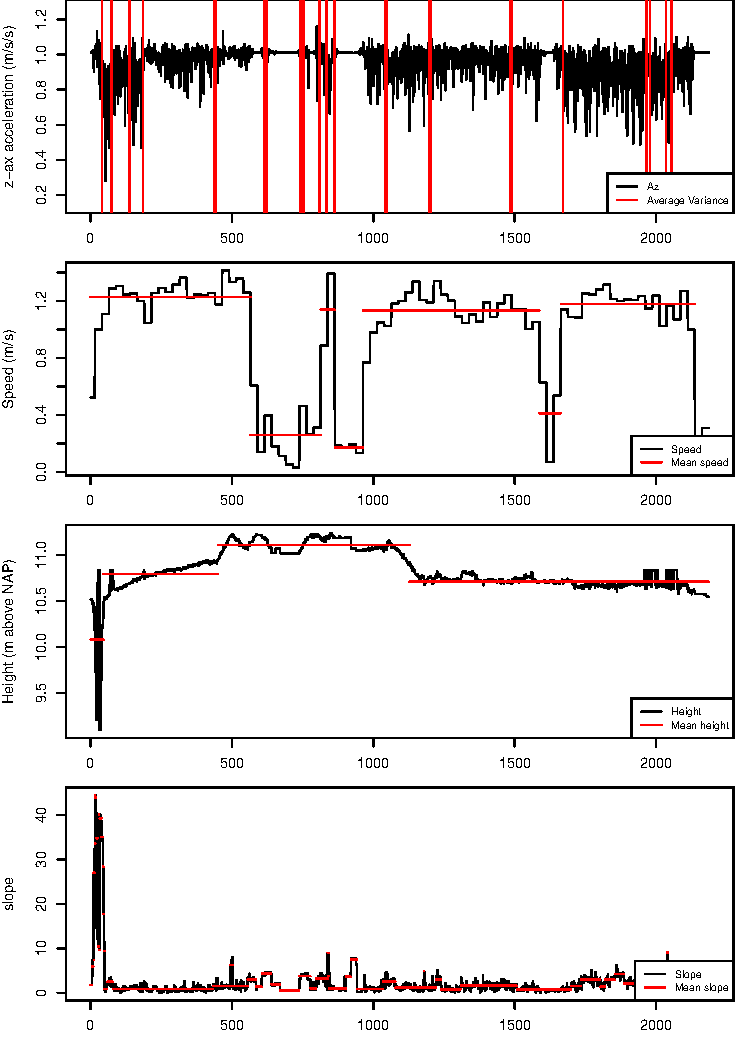
\includegraphics[ width=\textwidth]{img/R_ChangePointComparisonmeetr.pdf}
\centering
\caption{Changepoint segments per dataset of the MeetRollator route.\label{routeR}}
\end{figure} 





\clearpage

\subsection{changepoint and Segments found for the Leica walking route (without accelerometer)}
From the failed measurements there was one route walked with a Leica system. Though, there are no accelerometer measurements available for this route, the GPS-location is more accurate and the comparison of slope and speed could potentially give better results. 


\begin{figure}[ht]
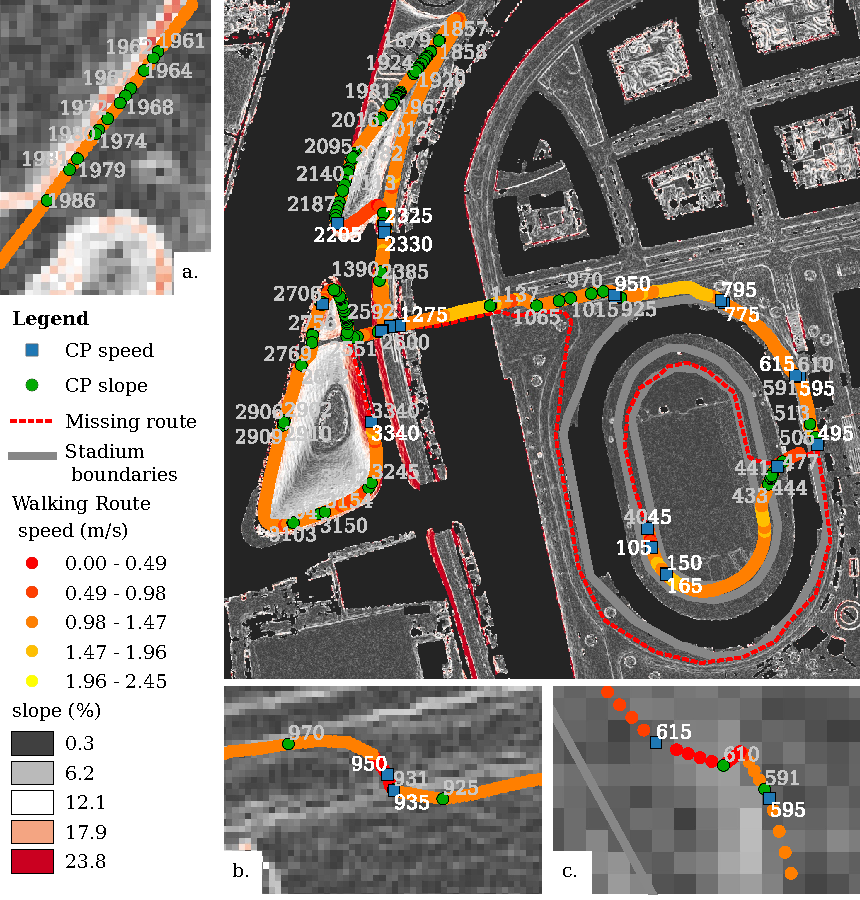
\includegraphics[width=\textwidth]{img/R_leicaroute.pdf}
\centering
\caption{Map with changepoints in speed and slope for the Leica route.\label{routeLeicaMap}}
\end{figure}

Figure \ref{routeLeicaMap} shows the complete route, starting in the stadium, going outside to the park and returning to the stadium. The Leica measurements stopped halfway the route and was not noticed by the user. This part is indicated with the red dotted line. The start of the route shows three changepoints in speed, an increase from standing still to walking. For the rest, the part of the route on the athletics track did not show any irregularities in slope or speed. The first interesting point is shown in the detailed map (c). The participants walked on the bicycle lane and realized to go onto the pavement, which are separated by a curb. The participant clearly slowed down and took the obstacle. Both changepoints in the speed and slope enclose this curb challenge. 
The detailed map (b) also shows a change of road segments. Again showing the same pattern in speed. Slowing down the speed, taking the curb obstacle and increasing speed again. Only here the changepoints for slope are positioned outside the speed changepoints. Detailed map (a) shows a part of the route in the park with a grassy hill in the middle which is enclosed by walking paths. A lot of changepoints in the slope are detected because the position of the measured route is slightly off the path and located n the edge of the hill. Of course the participant did not walk with his rollator on the edge of the hill, but on the middle of the path. Therefore these changepoint can be labelled as wrongly classified. 

\begin{table}[h]
\centering
\caption{Summary of changepoint output and methods used, per dataset, for the Leica walking route.}
\label{leicaCP}
\begin{tabular}{|p{175.3pt}|p{100.3pt}|p{100.3pt}|}
\hline
.. & Slope & Speed \\
\hline 
changepoint type 	& Change in mean 	& Change in mean 	\\
Method of analysis	& PELT 				& PELT 				\\
Test Statistic 		& Normal 			& Normal 			\\
Type of penalty		& MBIC with value, 24.34118 & AIC with value, 4 \\
Minimum Segment Length	& 1 			& 1 				 \\
Maximum no. of cpts 	& Inf 			& Inf 			 \\
Number of changepoints 	& 123			& 20				 \\
\hline
\multicolumn{3}{|l|}{Created Using changepoint version 2.2 } \\
\hline
\end{tabular}
\end{table}

\begin{figure}[H]
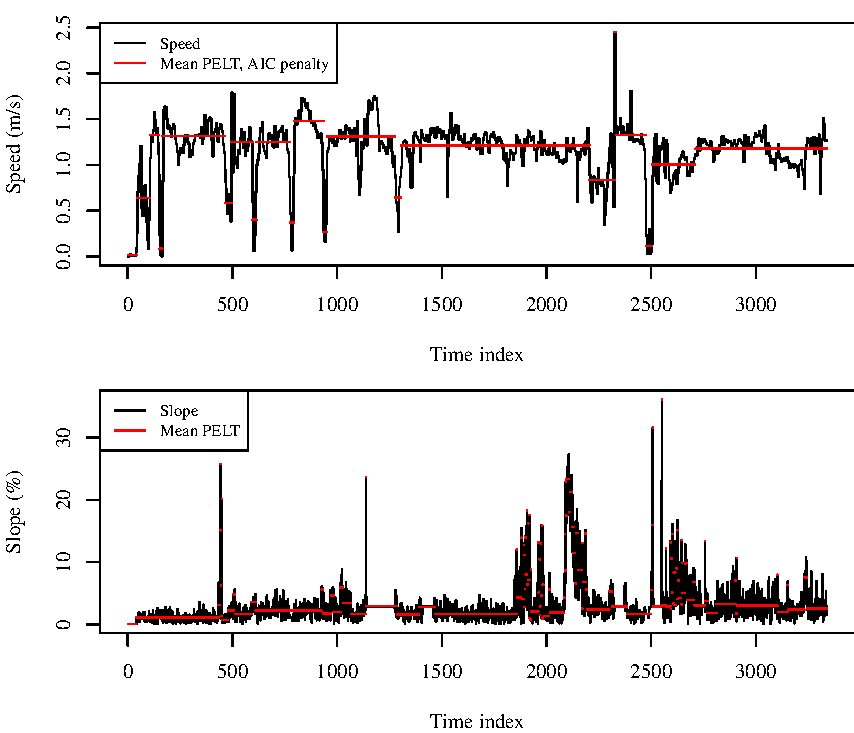
\includegraphics[width=\textwidth]{img/R_comparisonMethodsLeica.pdf}
\centering
\caption{Changepoint segments in speed and slope for the Leica route.\label{routeLeica}}
\end{figure} 



\clearpage

%Bike route
\subsection{changepoint and Segments found for the bike route}
For testing the accelerometer application, a route with GPS and the accelerometer app was conducted on the bike. This resulted into the following data. Figure \ref{routeB2} shows the route with the bike in the big top map. The left zoom squares (a) and (b) show a crossroad, where the bike path is interrupted by another type of road changing from concrete to tiled paving. As can be seen the speed shows changepoints before and after this crossing, where I slowed down with the bike to take the curves and check for upcoming traffic. Also a changepoint in the accelerometer is present, this could indicate the change of surface material and the little gap/border where the road sections change. We would have expected two changepoints, one going off the asphalt lane onto the crossing and one leaving the crossing going up the asphalt bicycle lane again. Unfortunately this is not the case. See figure \ref{crossroad} showing a Google street-view of the bicycle lane pavement changing to tiles at the crossing.

\begin{table}[!hb]
\centering
\caption{Summary of changepoint output and methods used, per dataset, for the cycle route.}
\label{sss}
\begin{tabular}{|p{109pt}|p{85pt}|p{85pt}|p{85pt}|}
	\hline
	.. & Slope & Speed & Variance z-axis \\
	\hline 
	Changepoint type 	& Change in mean 	& Change in mean 	& Change in variance \\
	Method of analysis	& PELT 				& PELT 				& PELT\\
	Test Statistic 		& Normal 			& Normal 			& Normal\\
	Type of penalty		& MBIC with value, 24.5802 & Manual with value, 12.2901 & Manual with value, 12.2901\\
	Minimum Segment Length	& 1 			& 1 				& 2 \\
	Maximum no. of cpts 	& Inf 			& Inf 			& Inf \\
	Number of changepoints 	& 195			& 27 				& 32 \\
	\hline
	\multicolumn{4}{|l|}{Created Using changepoint version 2.2 } \\
	\hline
\end{tabular}
\end{table}

\begin{figure}[hb]
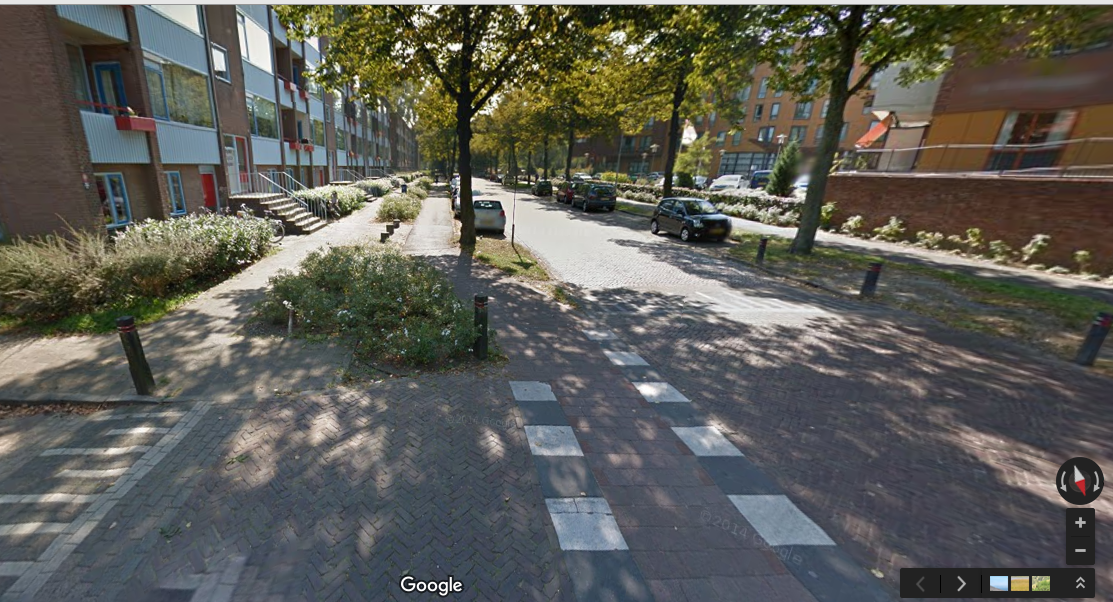
\includegraphics[width=\textwidth]{img/R_crossroad.png}
\centering
\caption{Google street-view of the cross road from map (b) figure \ref{routeB2}. \label{crossroad}}
\end{figure} 


The right square (c) shows a street with speed bumps that have to be crossed with the bike as well. The vertical acceleration changepoints indicate roughly these bumps and no change in speed is detected. Which is logical, because with a bike you do not really slow down for moderate speed bumps. A lot of changepoint in the slope come up but they do not indicate the speed bumps for the location was not accurate enough and the route is mapped next to the road several times. 



\begin{figure}[hb]
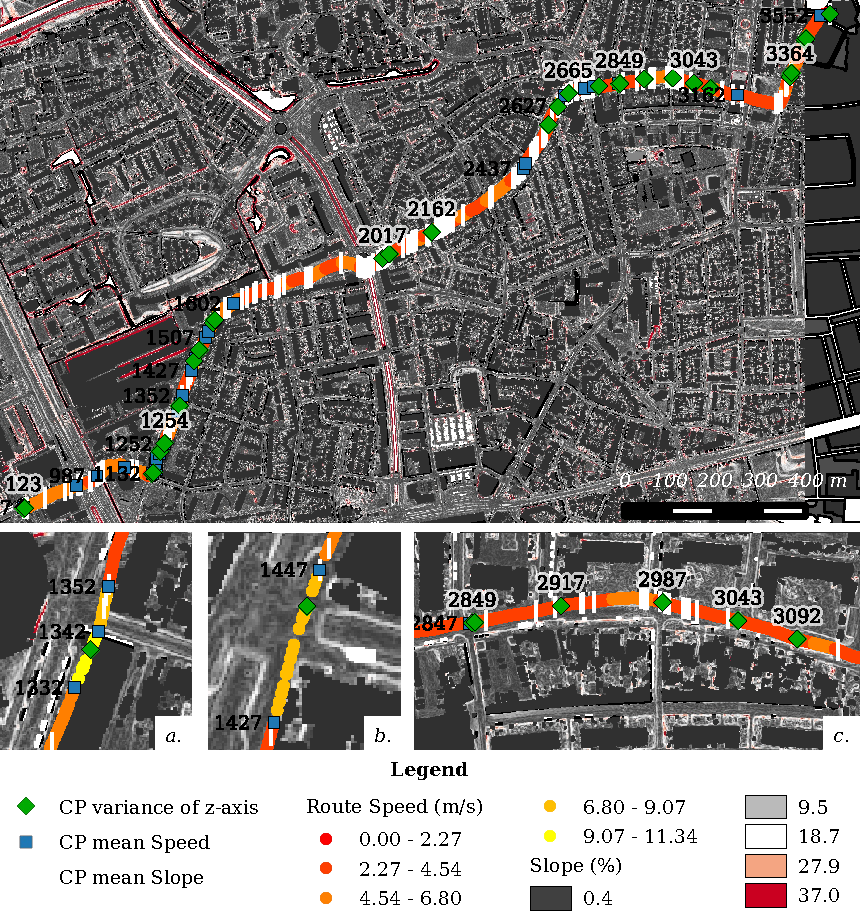
\includegraphics[width=\textwidth]{img/R_Bikeroute.pdf}
\centering
\caption{Map with changepoints of the bike route.\label{routeB2}}
\end{figure} 

\clearpage

\begin{figure}[ht]
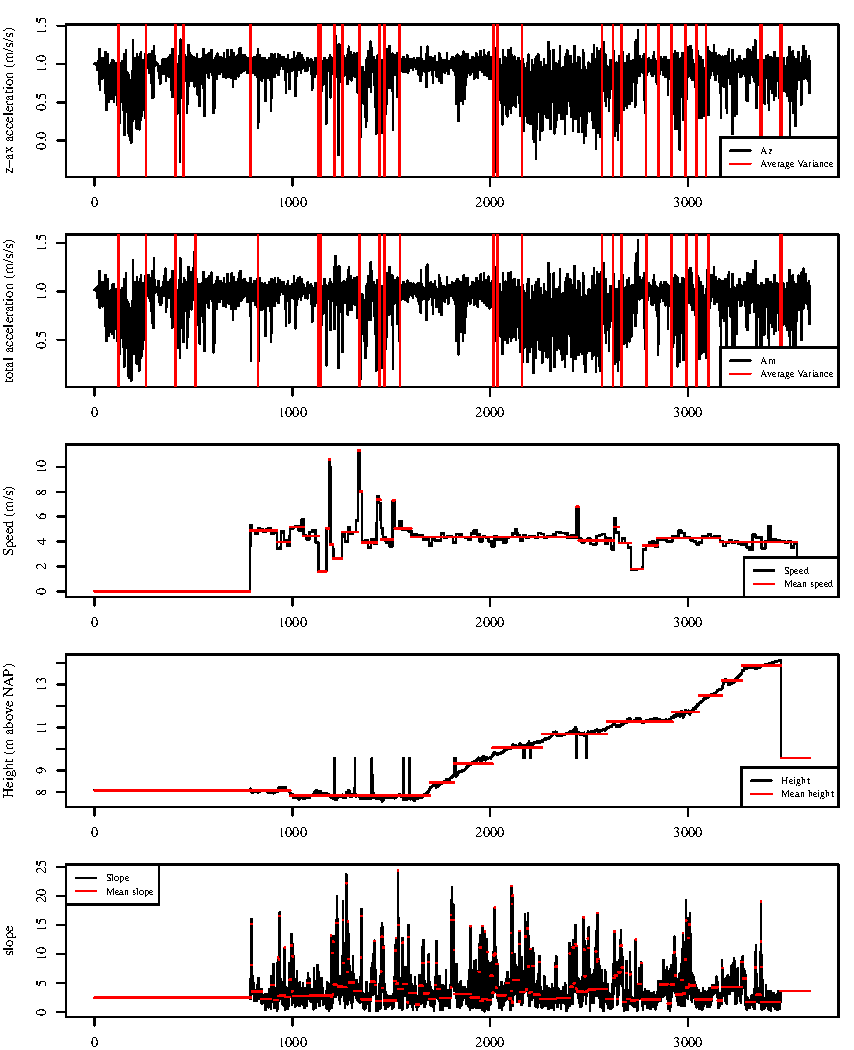
\includegraphics[width=\textwidth]{img/R_ChangePointComparisonbike.pdf}
\centering
\caption{Changepoint segments per dataset of the bike route.\label{routeB}}
\end{figure} 



\clearpage